%%%%%%%%%%%%%%%%%%%%%%% file typeinst.tex %%%%%%%%%%%%%%%%%%%%%%%%%
%
% This is the LaTeX source for the instructions to authors using
% the LaTeX document class 'llncs.cls' for contributions to
% the Lecture Notes in Computer Sciences series.
% http://www.springer.com/lncs       Springer Heidelberg 2006/05/04
%
% It may be used as a template for your own input - copy it
% to a new file with a new name and use it as the basis
% for your article.
%
% NB: the document class 'llncs' has its own and detailed documentation, see
% ftp://ftp.springer.de/data/pubftp/pub/tex/latex/llncs/latex2e/llncsdoc.pdf
%
%%%%%%%%%%%%%%%%%%%%%%%%%%%%%%%%%%%%%%%%%%%%%%%%%%%%%%%%%%%%%%%%%%%


\documentclass[runningheads,a4paper]{llncs}

\usepackage[latin1]{inputenc}
\usepackage{amssymb}
\setcounter{tocdepth}{3}
\usepackage{graphicx}
\usepackage{amsmath}
\usepackage{url}
\newcommand{\keywords}[1]{\par\addvspace\baselineskip
\noindent\keywordname\enspace\ignorespaces#1}

\begin{document}

\mainmatter  % start of an individual contribution

% first the title is needed
\title{Un marco de aplicaciones para computaci�n evolutiva voluntaria}

% a short form should be given in case it is too long for the running head
%\titlerunning{Lecture Notes in Computer Science: Authors' Instructions}

% the name(s) of the author(s) follow(s) next
%
<<<<<<< HEAD
\author{Israel Blancas \inst{1}\email{iblancasa@ugr.es}}
=======
\author{Israel Blancas \inst{1} \and J. J. Merelo \inst{1}}
>>>>>>> a9309e3fc72f6342b56bde5dbe4a00c2caa1bbdc
%
\authorrunning{La importancia de la computaci\'on voluntaria y un ejemplo}
% (feature abused for this document to repeat the title also on left hand pages)

% the affiliations are given next; don't give your e-mail address
% unless you accept that it will be published

\institute{Departamento de Arquitectura y Tecnolog\'ia de Computadores,
Universidad de Granada, Espa\~na}


\maketitle


\begin{abstract}
La computaci\'on voluntaria es una metodolog\'ia para realizar c\'alculos o procesamiento
de datos basado en la interconexi\'on de m\'ultiples clientes (que realizan el c\'omputo)
un servidor (que almacena los resultados y coordina los servidores). Frente a otros m\'etodos
de computaci\'on, la computaci\'on voluntaria brinda la oportunidad a los ciudadanos
de participar en experimentos cient\'ificos, aportando la potencia de sus m\'aquinas
para el tratamiento de los datos. Un ejemplo de ello es NodIO, un framework
que permite lanzar experimentos de computaci\'on voluntaria utilizando algoritmos
evolutivos. Este es desplegado sobre un PaaS (Platform as a Service -Plataforma como Servicio-)
y su principal ventaja radica en que est\'a escrito en Javascript, lo que permite
que una gran cantidad de dispositivos, sin depender de su arquitectura o de la
instalaci\'on de m\'as software que un navegador, pueda ejecutarlo y participar
en los distintos experimentos.
\end{abstract}


\begin{keywords}
  computaci\'on voluntaria, nodeo, nodio, algoritmos evolutivos, computaci\'on distribuida,
  computaci\'on internet, evaluaci\'on de rendimiento
\end{keywords}

\section{Motivaci\'on}
En este art\'iculo se pretende dar a conocer la computaci\'on voluntaria y
el framework de c\'odigo abierto llamado ``NodIO" \cite{nodio}, mediante el cual
se pueden lanzar experimentos de computaci\'on voluntaria
que permitan ejecutar algoritmos gen\'eticos (utilizando el framework NodEO \cite{nodeo}),
y ser ejecutados por los usuarios desde un navegador web.


\section{Introducci\'on}
%
Diversos son los m\'etodos utilizados por los llamados cient\'ificos
de datos para el procesamiento de largos conjuntos de resultados obtenidos
a trav\'es de la elaboraci\'on de experimentos o, en su defecto, la propia
realizaci\'on de los experimentos: uso de un \'unico supercomputador para
todo el procesamiento; creaci\'on de un cl\'uster de m\'aquinas en un centro
de procesamiento (o cloud); o, como en el caso que nos ocupa, la computaci\'on voluntaria.

\subsection{Computaci\'on voluntaria}
La computaci\'on voluntaria es un m\'etodo de c\'omputo mediante el cual se
permite a distintos usuarios colaborar en un proyecto cient\'ifico,
en muchas ocasiones, aprovechando el tiempo ocioso de sus m\'aquinas. Esta colaboraci\'on
se produce entre computadores independientes, interconectados a trav\'es de una o varias redes
para comunicar informaci\'on y coordinar sus tareas construyendo redes con potencias
equivalentes a la de los supercomputadores o, incluso, superiores.

Ejemplos de ello son los descritos en \cite{seti} o \cite{climate}, sistemas creados por
departamentos de universidades para la realizaci\'on de m\'ultiples estudios
(cabe destacar que este tipo de iniciativas suelen estar impulsadas por
instituciones acad\'emicas), aunque el primero fue ``Great Internet Mersenne Prime Search" en 1996,
un sistema para buscar n\'umeros primos de Mersenne \cite{gimps}.

En estos sistemas se desean las siguientes caracter\'isticas:
\begin{itemize}
  \item Tolerancia a fallos: en caso que una de las m\'aquinas deje de hacer un trabajo, es
  conveniente que se ese c\'omputo sea realizado por otro usuario
  \item Seguridad: para evitar que un usuario nocivo (o varios) puedan causar alg\'un da\~no
  al resto
  \item Ejecuci\'on en m\'ultiples m\'aquinas (incluso m\'aquinas de distinta naturaleza):
  si el experimento o la transformaci\'on de los datos no se realiza en un n\'umero suficiente
  de m\'aquinas, no se tendr\'a potencia de c\'alculo para obtener resultados fruct\'iferos
  \item Compatibilidad entre los dispositivos conectados: es necesario que
  las distintas m\'aquinas puedan entenderse entre ellas, de forma que el resultado
  de una pueda ser interpretado por otra
  \item Escalable: que el sistema sea escalable es un punto muy importante, ya que
  cuanto mayor sea la escalabilidad, mayor ser\'a la potencia de c\'omputo. Adem\'as,
  se debe garantizar que el sistema no tenga fallos debido al aumento del n\'umero de
  usuarios conectados
\end{itemize}

La potencia computacional total del sistema variar\'a en funci\'on del n\'umero de
usuarios que decidan colaborar, as\'i como de la propia potencia de sus m\'aquinas
y la capacidad del nodo ``coordinador" sistema para repartir el trabajo
y recoger los resultados.

La computaci\'on voluntaria es importante, entre otras de las cuestiones ya expuestas,
porque permite que ciudadanos fuera del \'ambito de la investigaci\'on, puedan
tomar parte de la misma.

Adem\'as, gracias a que son los usuarios quienes ``prestan" sus m\'aquinas, el sistema
es m\'as barato que la contrataci\'on de c\'omputo o la compra de material dedicado.

Por su contra, la dificultad para llegar a un n\'umero importante de gente y los posibles
problemas que pueden aparecer en cuanto a la fiabilidad o correcci\'on de los datos
(aunque se pueden establecer mecanismos como la computaci\'on redundante
para asegurar la correcci\'on o la firma de c\'odigo para prevenir modificaciones maliciosas
del software), hacen que el m\'etodo no sea ideal.

En estos sistemas, los usuarios depositan su confianza en el proyecto, suponiendo que:
\begin{itemize}
  \item El software que est\'an ejecutando no da\~na sus dispositivos
  \item El c\'omputo que se est\'a realizando servir\'a para la cuesti\'on que se
  ha anunciado y c\'omo se tratar\'a la propiedad intelectual de los resultados
  \item El sistema est\'a blindado contra usuarios maliciosos, evitando que
  se convierta en un canal para llevar a cabo actividades il\'icitas
\end{itemize}

\section{NodIO}
\subsection{\textquestiondown	Qu\'e es NodIO?}
NodIO \cite{nodio} es un software desarrollado para ser desplegado en un
Plataforma como Servicio (Platform A a Service), que, a su vez, se basa en un
framework llamado NodEO, pensado para el desarrollo de algoritmos gen\'eticos,
desarrollado en NodeJS.

Gracias a esta implementaci\'on, se pueden lanzar experimentos y ejecutarlos a
trav\'es de un navegador (o cualquier sistema que ejecute el lenguaje Javascript
y que disponga de conexi\'on a Internet)
por cada uno de los usuarios que accedan al servidor.


\subsection{Funcionamiento}
\subsubsection{Arquitectura}
Este sistema cloud sigue un paradigma cliente - servidor:
\begin{itemize}
  \item Servidor: realiza la coordinaci\'on de los clientes, almacena los distintos chromosomas y
  el estado de los experimentos y reinicia el experimento cuando se ha encontrado la soluci\'on.
  El acceso y env\'io de los distintos chromosomas se hace a trav'es de una interfaz API/REST.
  Las peticiones (que siguen el ciclo ``CRUD") utilizan el formato JSON. Est\'a escrito en NodeJS.
  \item Cliente: procede con el c\'omputo. Hace peticiones as\'incronas al servidor.
  En aquellos navegadores en los que est\'e permitido, se ejecuta utilizando ``Web Workers"
  (en caso contrario, se ejecuta una versi\'on preparada para ello). Est\'a escrito
  en Javascript, ya que se dise\~n\'o pensando en que fuese ejecutado en navegadores aunque
  (gracias a que el servidor utiliza una API/REST), se podr\'ia escribir en cualquier otro
  lenguaje, siendo totalmente compatible con el actual servidor.
\end{itemize}



\subsubsection{Env\'io de mensajes y coordinaci\'on}
Como se ha mencionado anteriormente, el sistema NodIO se basa en NodEO, que permite la
ejecuci\'on de algoritmos gen\'eticos escritos en Javascript. El sistema procede
de la siguiente forma:
\begin{enumerate}
  \item El servidor es iniciado. Se inicializa un conjunto aleatorio de chromosomas,
  que llamaremos ``poblaci\'on compartida"
  \item Cada cliente se conecta al servidor y se le env\'ia la web y los scripts asociados
  \item Se asigna a cada cliente un UUID
  \item Cada cliente recibe un chromosoma aleatorio
  \item Se comienza con los c\'alculos
  y ejecuta N generaciones
  \item Actualizaci\'on de las gr\'aficas de la web
  \item Cada cliente env\'ia el mejor individuo al servidor, que guarda en la poblaci\'on compartida
  \begin{enumerate}
    \item Si el chromosoma enviado no es el mejor global:
      \begin{enumerate}
        \item Se recibe un individuo de la poblaci\'on compartida
        \item Vuelta al quinto paso
      \end{enumerate}
    \item Si el chromosoma es el mejor global:
      \begin{enumerate}
        \item Incremento del n\'umero de secuencia en el servidor
        \item Reseteo de la poblaci\'on compartida
        \item Se inicia un nuevo experimento
        \item Reseteo del UUID
        \item Vuelta al cuarto paso
      \end{enumerate}
  \end{enumerate}
\end{enumerate}

\subsubsection{Crear un nuevo experimento}
La creaci\'on de un nuevo exprimento se basa en la modificaci\'on de algunos archivos.
Principalmente:
\begin{itemize}
  \item \textbf{is\_solution.js}: este fichero, que se ejecuta en el servidor,
  decide si la soluci\'on enviada por el cliente es v\'alida, es decir,
  comprueba que se haya alcanzado la soluci\'on y, en caso afirmativo, se
  aumenta el n\'umero de secuencia y se comienza de nuevo. Cuando se desee
  crear un nuevo experimento, ser\'a necesario reescribir esta funci\'on y
  adecuarlo a las caracter\'isticas de la nueva.
  \item \textbf{trap.standalone.js}: este archivo se encuentra y ejecuta en el cliente.
  Sirve como base a un nuevo desarrollo. Contiene las funciones necesarias para
  el dibujado de las gr\'aficas y la evaluaci\'on y generaci\'on de los individuos.
  Aqu\'i es donde crearemos una funci\'on que eval\'ue el fitness de cada uno de
  los chromosomas generados. No olvidemos que NodIO hace uso de la biblioteca
  NodEO \cite{nodeo}, lo que quiere decir que algunas de las funciones que vemos en
  \textit{trap.standalone.js} est\'an definidas en NodEO (aunque podr\'iamos prescindir
  de este framework e implementar las nuestras propias).
\end{itemize}

Dependiendo de las necesidades que tenga el experimento deseado, ser\'a necesaria
la revisi\'on de otros archivos para ajustar aquellos par\'ametros que se deseen.
Esto no es problema al contar NodIO con una licencia libre.

\subsection{Experimentos}

\subsubsection{Comprobando la reducci\'on de tiempo a mayor n\'umero de pesta\~nas}.
Como se dec\'ia cuando se introduc\'ia a la computaci\'on voluntaria,
el uso de muchos dispositivos, convierte el sistema en una gran red computacional.
Esto nos permite resolver problemas que ser\'ian demasiado costosos para una sola
m\'aquina mucho m\'as r\'apido. Por este motivo, utilizando el experimento
en el que se resuelve la ``funci\'on trap", se desea
demostrar, a muy peque\~na escala, c\'omo de beneficiosa puede llegar a ser la computaci\'on
voluntaria para obtener resultados.

Las variables pasan a tomar los siguientes valores:
\begin{itemize}
  \item traps: 24
  \item longitud trap: 4
  \item b: 2
  \item cach\'e: 32
  \item tama\~no problaci\'on: 128
\end{itemize}

Estos valores son los mismos que los vistos en el anterior experimento, excepto
el n\'umero de traps, que se ha reducido para obtener un problema suficientemente
complejo para realizar algo de c\'omputo pero no demasiado lento para poder hacer
muchas mediciones (el valor se ha obtenido de forma emp\'irica).

Tras esto, se ha procedido a poner en marcha el servidor y ejecutar los algoritmos
variando el n\'umero de pesta\~nas abiertas en el navegador. Los resultados
se pueden observar en la figura \ref{tiempo-pestanas}.

\begin{figure}[htbp]
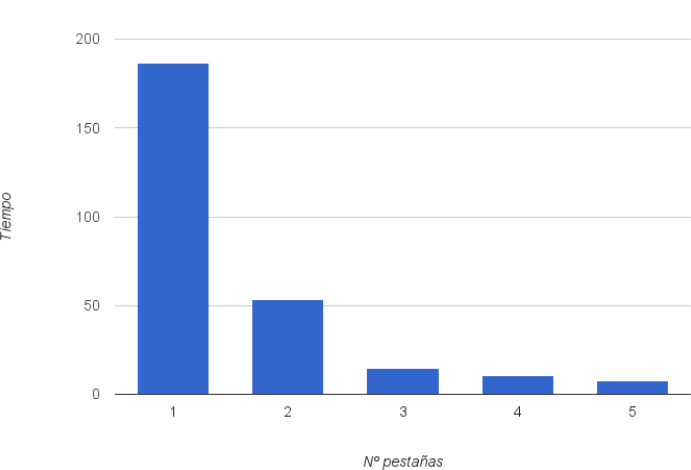
\includegraphics[scale=0.6]{img/tiempo-pestanas}
\centering
\caption{Resultados obtenidos al medir el tiempo que se tarda en alcanzar una
soluci\'on en un mismo ordenador en funci\'on del n\'umero de pesta\~nas abierto}
\label{tiempo-pestanas}
\end{figure}

Estas pruebas se han hecho en un sistema operativo GNU/Linux (distribuci\'on ArchLinux con
kernel 4.5.1) con un procesador i5-2410M CPU @ 2.30GHz. El navegador utilizado ha sido la
versi\'on 50 de Chromium.

Como podemos observar, cuando solo tenemos una pesta\~na abierta, el tiempo se
dispara (en torno a unos 3 minutos). En el caso de dos pesta\~nas, el tiempo descenci\'o hasta
un tiempo estimado a los 53.22 segundos. En el resto de los casos, aunque sigue habiendo
diferencias de tiempo (unos 14.56, 10.11 y 7.46 segundos respectivamente), no es
tan notable como en los otros dos casos. Esto puede tener varias explicaciones: por un
lado al aumentar el n\'umero de pesta\~nas, el poder computacional desciende (el
sistema operativo se ve con una carga de trabajo con la que tiene que lidiar).
Por otro, llegar\'a un momento en el que no se podr\'a reducir m\'as el tiempo
de ejecuci\'on por la propia naturaleza del problema.


\subsubsection{Comprobando la reducci\'on de tiempo utilizando varios dispositivos del mismo modelo.}

En esta ocasi\'on, utilizando exactamente la misma versi\'on del software que en
el experimento anterior (el mismo cliente y el mismo servidor utilizando los mismos valores),
se ha procedido a medir los tiempos ejecuci\'on en varios dispositivos (siendo el mismo
modelo hardware -tel\'efonos m\'oviles LG Bello II, con procesador quad-core
Cortex-A7 1.3GHz-, navegador -Chrome- y la misma versi\'on Android -5.0.2-).

En la figura \ref{tiempo-dispositivos} podemos ver los resultados.  Si comparamos con
la figura \ref{tiempo-pestanas}, es sencillo ver que existe una simetr\'ia, aunque
en este nuevo caso los tiempos son algo mayores (que podemos achacar a un menor rendimiento
por parte del procesador del dispositivo m\'ovil y a la existencia de una red entre
el servidor y los dispositivos, cuando antes se ejecutaba todo dentro de la misma
m\'aquina).

\begin{figure}[htbp]
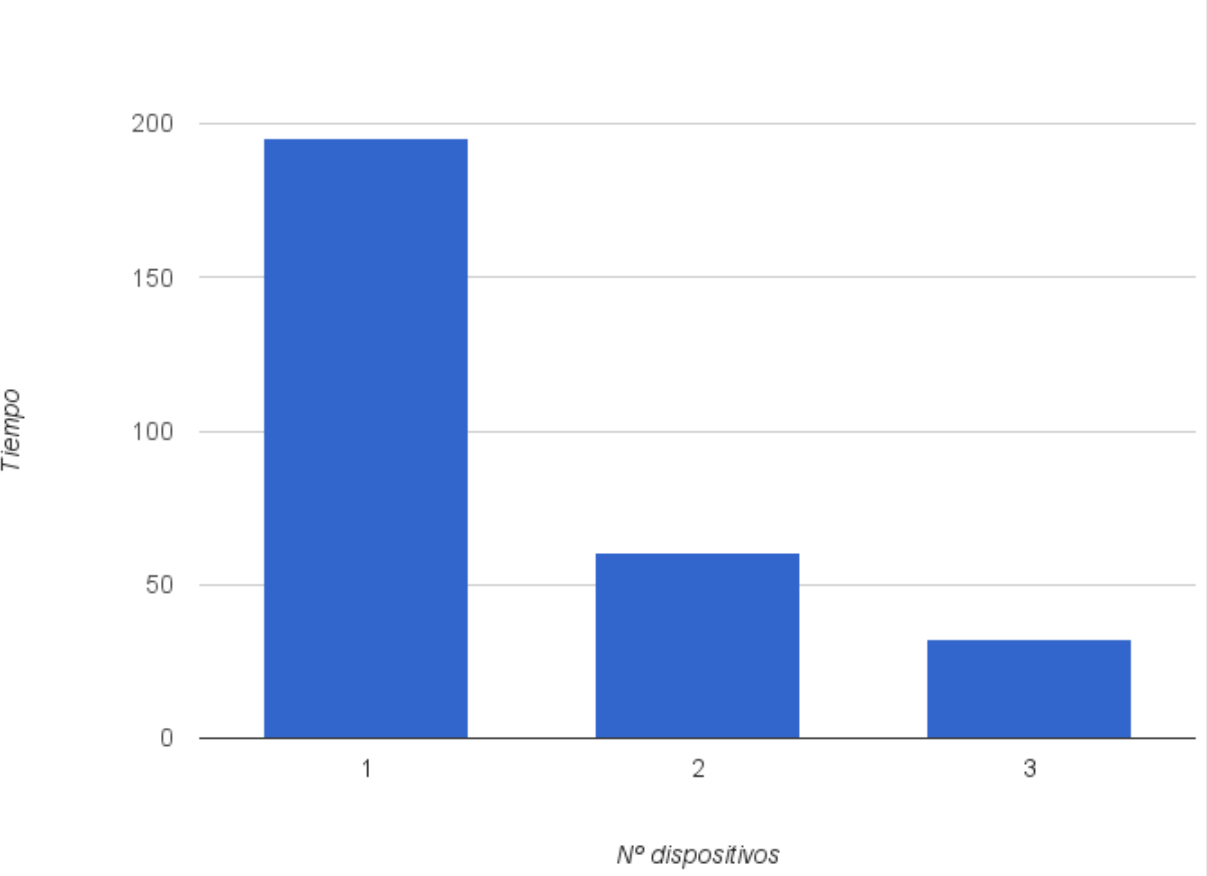
\includegraphics[scale=0.6]{img/tiempo-dispositivos}
\centering
\caption{Resultados obtenidos al medir el tiempo que se tarda en alcanzar una
soluci\'on utilizando varios dispositivos con la misma configuraci\'on hardware y software}
\label{tiempo-dispositivos}
\end{figure}




\subsection{Trabajos futuros}
Muchas son las ideas que se pueden desarrollar utilizando esta herramienta (o a
partir de la misma). Aqu\'i se destacar\'an:
\begin{itemize}
  \item Realizaci\'on de nuevos experimentos: teniendo en cuenta los experimentos
  que ya se realizaron en \cite{nodio} o los que se presentan en las anteriores l\'ineas,
  un experimento interesante podr\'ia ser medir la velocidad de ejecuci\'on del
  mismo software utilizando dispositivos de distinta potencia (para comprobar
  si esto afecta mucho o no a la ejecuci\'on del c\'odigo Javascript).
  \item Facilitar la creaci\'on de nuevos experimentos: actualmente, tener que cambiar
  varios ficheros puede ser una tarea engorrosa y ser\'ia un cometido a tener en cuenta el
  facilitaci\'on de la misma. Adem\'as ser\'ia \'util (para
  aquellos usuarios que no se encuentren familizarizados con Javascript o simplemente
  no quieran reescribir su c\'odigo), la
  integraci\'on de forma sencilla de conversores de c\'odigo (como es el caso de ScalaJS,
  que permite ``traducir" c\'odigo escrito en lenguaje Scala a Javascript).
  \item Aplicar t\'ecnicas de ``gamificaci\'on": probablemente podamos sacar
  provecho a la ludificaci\'on para atraer a m\'as usuarios (y durante m\'as tiempo)
  para que participen en los experimentos. Un ranking por puntos o alg\'un tipo de
  bonificaci\'on podr\'ian hacer que los resultados (y sobre todo los tiempos de
  ejecuci\'on) mejorasen notablemente.
  \item Soporte a m\'ultiples idiomas: actualmente la p\'agina donde se realizan los
  experimentos est\'a en ingl\'es. Si se proporcina soporte a distintos idiomas,
  ser\'a m\'as sencillo captar nuevos usuarios (m\'as teniendo en cuenta que,
  cuando se lanza el experimento, la difusi\'on de la web se realiza mediante
  redes sociales en perfiles de habla hispana).
\end{itemize}



\bibliographystyle{splncs}
\bibliography{volunteer}

\end{document}
